% 一、立项依据：研究目的、意义及应用前景，国内外研究概况。
% 内容迁自 NSFC_2026_MineChangeTrust；保留原稿事实、暂定值和待补项。
\subsection{研究背景与意义}
% 原稿关于借用 NSFC 正文版式的工作稿说明不再作为目标正文显示。

矿山开采、堆置与复垦会改变地表覆盖及其空间边界。遥感影像能够提供跨区域的地表观测，但要把两期影像中的差异转化为可供复核的变化范围，还需区分真实地物变化与光照、地表湿度、植被状态等外观差异。全球矿山用地数据已使矿业活动的空间分布获得较系统的刻画\cite{Maus2020Mining,Maus2022Mining}；矿山变化检测进一步把研究对象从单期范围识别推进到两期变化定位\cite{Yu2024MineNetCD}。对矿山地质环境监测而言，清楚标示何处发生可观测变化、哪些判断容易出错，有助于减少逐幅筛查的工作量，也为后续专业解释提供可追溯的影像线索。

本课题“矿山地表扰动遥感变化检测的跨域泛化与可信评估研究”面向中南大学有色金属成矿预测与地质环境监测教育部重点实验室开放课题的矿山地质环境监测方向，研究公开影像及变化标签能够支持的地表覆盖和矿山足迹变化。“跨域泛化”主要指模型在未参与训练、选择及校准的矿区上保持判别能力；“可信评估”关注预测概率与实际错误是否相符、能否识别错误区域，以及固定工作量下的复核效用。污染程度、沉降风险或生态修复成效的判定需要相应观测与专业证据，仅凭二值变化标注无法作出这些判断。

矿区之间的地貌、背景地物和观测条件差异，为变化检测带来两类相互关联的问题。其一，背景外观发生差异时，模型可能产生误报；对跨时相特征施加过强的一致性要求，又可能削弱真实细小变化。其二，即使平均检测指标尚可，模型仍可能在部分新矿区给出高置信度错误。若复核只依据预测变化区或最高不确定区域，模型确信“未变化”的漏检会被遗漏。本课题将通过分组对照和具体误报、漏检案例，分析约束区域及其适用条件，并检验有限复核面积内能够发现哪些错误。

上述研究需求及两类差异的关系如图\ref{fig:mct-background}所示。
\begin{center}
\begin{minipage}{\linewidth}
  \centering
  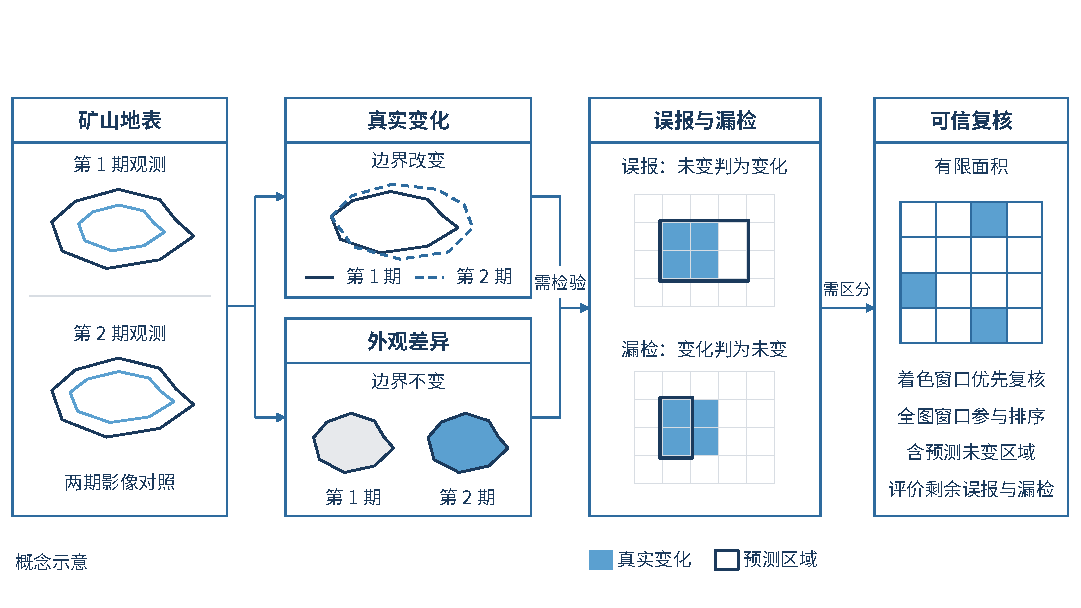
\includegraphics[width=\linewidth,trim=0 0 0 12mm,clip]{figures/vector/F01_research_background.pdf}
  \captionsetup{justification=justified,singlelinecheck=false}
  \captionof{figure}{研究背景：真实地表变化、外观差异与复核需求。场景、轮廓与复核过程均为概念示意，用于说明需要区分的观测差异与错误，不表示已验证的误差归因。}
  \label{fig:mct-background}
\end{minipage}
\end{center}

\subsection{国内外研究现状及发展动态分析}
\textbf{（1）矿山公开数据正在从范围制图走向变化及年度足迹分析。}
MineNetCD覆盖100个全球矿区，包含超过7万对双时相切片及像素级变化标注，并提供ChangeFFT等基准配置。其原论文已按矿区以60\%/10\%/30\%划分训练、验证与测试\cite{Yu2024MineNetCD}，因此矿区隔离本身是本研究应沿用的评测基础。该数据的时相间隔较长，适合研究两期之间的变化范围，不能据此开展逐月事件定位或实时预警。EuroMineNet进一步提供欧盟133个矿区2015—2024年的Sentinel-2年度观测与足迹标签，也采用矿区分组划分\cite{Yu2026EuroMineNet}。两者的分辨率、波段、时相间隔和标签含义存在差别，直接比较其变化交并比（IoU）不能单独解释域偏移。全球铜矿边界与属性数据可辅助核对有色金属矿案例\cite{Li2025Copper}，但单期边界不能充当双时相变化真值。

\textbf{（2）变化检测已形成多类表征方法，约束区域的作用仍需针对性检验。}
早期全卷积孪生网络通过双分支特征差异实现变化定位\cite{Daudt2018Siamese}。SNUNet-CD利用密集连接与多尺度交互\cite{Fang2022SNUNet}，BIT与ChangeFormer分别探索语义标记建模及层次Transformer结构\cite{Chen2022BIT,Bandara2022ChangeFormer}，ChangeMamba将状态空间建模用于遥感变化检测\cite{Chen2024ChangeMamba}。这些方法可作为骨干与比较对象。比较时需控制模型容量、上下文范围和训练配置，以判断性能差异是否来自本课题所研究的方法。

与本项目最接近的工作已涉及一致性和域泛化。FCCDN通过特征约束促进变化判别\cite{Chen2022FCCDN}；DonaNet结合域风格处理、跨时相风格变换及一致性学习，旨在缓解伪变化与跨域泛化问题\cite{Zang2025DonaNet}；CDDGNet进一步研究变化信息与域信息的解耦\cite{Zhao2026CDDG}。在已有泛化变化检测、特征约束和域特征解耦研究的基础上，本课题进一步检验：当一致性约束覆盖真实变化像素时，是否出现可测量的变化敏感性损失；把约束限定于训练标签确认的稳定区，能否在特定干扰条件下缓解这一损失。对此需要分别控制约束面积、强度、空间形状和平滑效应，仅凭增加一个掩码后总体分数上升，还无法判断收益是否来自约束区域的改变。

\textbf{（3）跨域研究要求区分泛化、适应与评测选择。}
通用域泛化研究说明，模型选择与评估协议会影响方法比较，简单基线和一致的选择规则不可省略\cite{Gulrajani2021DomainBed}；MixStyle从特征统计混合研究外观变化的表征学习\cite{Zhou2021MixStyle}，WILDS则通过现实分布变化任务强调域偏移的多样性\cite{Koh2021WILDS}。在遥感变化检测中，AWDA使用目标域无标签数据进行适应\cite{AWDA2025}，其可用信息与不接触目标域数据的纯泛化不同。本项目按可用训练信息分组报告结果，仅在信息条件一致的组内比较方法优劣。

空间数据还存在相邻样本依赖。相关研究讨论了结构化交叉验证、空间预测与插值/外推目标之间的关系\cite{Roberts2017CV,Valavi2019BlockCV,Mila2022Nearest}；遥感制图实例显示，验证方式可能显著影响所报告的预测表现\cite{Ploton2020Spatial}。这些证据支持本课题审计矿区、场景和切片来源，但不能用来指认MineNetCD官方划分已经泄漏。拟分别保留官方协议复现结果与新增校准划分下的结果，所有主比较方法共享相同的训练、选择及测试矿区。

\textbf{（4）校准质量与复核价值需要分别验证。}
温度缩放可作为深度网络概率校准的简单基线\cite{Guo2017Calibration}。分布偏移下的不确定性研究表明，源分布表现不能保证新分布上的可靠性\cite{Ovadia2019Uncertainty}；模型架构与校准之间的关系较为复杂，不能概括为“模型越新越不可靠”\cite{Minderer2021Calibration}。遥感变化检测已有利用不确定性描述或改进预测的工作\cite{Li2025Uncertainty}，本课题需进一步检验这些信息能否帮助发现错误。温度缩放改变概率尺度，在一些排序定义下未必改变样本顺序；因此，分别评价概率误差是否下降、错误排序是否改善。

选择性预测通过接受或拒绝部分结果研究风险与覆盖之间的关系\cite{Geifman2019SelectiveNet,Gangrade2021Selective,Franc2023Reject}。这一思路可用于组织人工复核，但像素分类风险与真实复核工作量并不等价：邻近错误可能集中在同一窗口，零散错误则可能需要多次查看；仅报告保留区准确率还可能掩盖未选中区域的漏检。矿山变化复核应在整幅有效区域上分配固定面积预算，同时报告误报、漏检与真实变化覆盖，才能判断排序信息是否具有使用价值。

\subsection{现有研究的不足}
\textbf{第一，一致性约束的收益与损伤还需在矿山任务中分开识别。}
已有工作给出通用约束方法，但其总体指标难以说明本课题数据中的误差有多少来自背景外观，有多少来自真实变化的特征收缩。单一IoU合并误报与漏检，且受变化占比影响，难以单独识别细小变化损失。本课题分别控制约束区域和强度，补充判决阈值敏感性分析，再按变化尺度与外观差异分层。分层结果用于描述条件关联，受控对照用于排查替代解释。

\textbf{第二，可靠性改善能否转化为复核收益仍需直接证据。}
概率校准误差、错误排序和人工复核分别回答不同问题。现有概念与方法不能自动保证新矿区高置信度漏检被发现。需要用包含预测未变化区的统一窗口集合，比较随机、原始熵、校准熵及推理分歧在同等面积下留下的错误，明确理想纠错模拟与真实人员复核的差别。

\textbf{第三，矿山场景中的方法结论需要具有可追溯的外部有效性边界。}
矿区隔离、标签口径和输入适配是建立可信结论的基础。泛化优势若只来自少数大矿区、特定变化尺度或某种标注方式，其适用范围应如实报告。本课题重点考察哪些条件下能够重现结果、哪些矿区会出现反例；跨数据集比较须先对齐输入与标签含义。

\subsection{关键科学问题与研究切入点}
本项目的中心问题是：\textbf{一致性约束的空间分配能否缓解未见矿区中背景误报与细小变化漏检的权衡？}重点区分三种解释：约束区域改变了变化判别；总体约束变弱；预测分数移动使固定阈值下的检出减少。可靠性评价作为辅助研究，进一步检查约束后残留的错误能否被排序发现。

待检验的核心假说为：在训练监督及计算预算一致的条件下，背景限定约束相对全图约束可减少误报，并保持细小变化召回非劣。联合收益还须经随机掩码、强度、平滑及阈值对照解释；若收益由这些因素解释，或召回损失超过非劣界，则不支持区域选择的解释。相对全图有利仅说明两种约束存在相对差异；是否减轻损伤、是否产生新增收益，须结合无约束组判断。稳定背景仅指训练标签确认未变化的区域，不预设地质稳定性。

辅助假说为：在独立矿区校准和开发集选择之后，固定多视图推理分歧与概率熵的简洁组合，能够在固定复核面积内比单独指标发现更多错误，并降低未复核区域漏检。其有效性用全图剩余误报和漏检分别检验；优势若仅出现在高复核比例或单个矿区，不扩大为普遍可靠性结论。

已在MineNetCD裁切子样本上完成三组、三个种子的预实验，详见研究基础。背景约束相对全图的降误报伴随总体召回下降，IoU差区间跨零，小变化端点不可估计，尚不支持联合假说。该权衡正是后续对照需要解释的现象：先核验来源、配准和小变化样本，再判断它来自区域选择、约束强度还是分数尺度。无论联合收益是否成立，均形成可复核的效应范围与反例；不以重新选择指标替代假说检验。
